\documentclass{article}
\textwidth=6in
\hoffset=0in
\voffset=0in

\usepackage[a4paper, total={6in, 8in}]{geometry}
\usepackage{amsmath}
\usepackage{amssymb}
\usepackage{stmaryrd}
\usepackage{graphicx}
\usepackage{tikz}
\usetikzlibrary{automata, arrows}
\usepackage{pifont}
\usepackage{amssymb}
\usepackage{gensymb}
\usepackage[ampersand]{easylist}

% needs to be updated
\author{Max Springenberg, 177792}
\title{\
    GTI Uebungsblatt 1
    }
\setcounter{section}{1}
\date{}

% custom commands
% \Theta \Omega \omega
\newcommand{\tab}{\null\ \qquad}
\newcommand{\gap}{\null\ \\ \\}
\newcommand{\lA}{\leftarrow}
\newcommand{\rA}{\rightarrow}
\newcommand{\ue}{\infty}
\newcommand{\eps}{\epsilon}
\newcommand{\task}[1]{\textbf{#1} \\ \gap}
\newcommand{\cmark}{\ding{51}}
\newcommand{\xmark}{\ding{55}}
\newcommand {\degr}{\degree}

% content
\begin{document}
% title page
\maketitle
\newpage
% actual paper
\subsection\
\subsubsection{\
    Wie wandelt man einen NFA mit $\eps$-Übergängen in einen äquivalenten 
        NFA ohne solche Übergänge um?
    }
In der Vorlesung wurde die $\eps$-closure Funktion vorgestellt, die fuer einem 
    Zustand die Menge aller Zustaende die mit $\eps$ von diesem aus erreichbar
    sind zuordnet.\\
Unter der Verwendung dieser Fuinktion lassen sich mehrere Zustaende zu einem
    zusammenfassen. Dabei werden die transitionen aller Zustaende, die zusammen
    gefasst wurden aufrecht erhalten.\\
\subsubsection{\
    Sei L eine reguläre Sprache über einem Alphabet $\Sigma$, und sei 
        $A = (Q, \Sigma, \delta, s, F)$ ein NFA, der diese Sprache entscheidet.
        Wir definieren die Präfix-Sprache $prep(L)$ wie folgt:\[
            pre(L) = \{v \in \Sigma^* | \exists x \in L : vx \in L\}
        \]
    }
\task{\
    (a) Konstruieren Sie einen NFA $A_p = (Q,\Sigma,\delta,s,F_p)$ fuer die Sprache
        $pre(L)$, indem Sie die Menge $F_p$ der akzeptierenden Zustaende von
        $A_p$ bestimmen.
    }
Der Automat akzeptiert fuer aller Woerter, die Praefix eines Wortes in L sind.\\
Fuer alle Woerter in L gilt, dass die Eingabe ihrer Zeichen in einem
    akzeptierendem Zustand endet. Ferner gilt das fuer jeden ihrer Prefixe ein
    Lauf zu diesem Wort existiert.\\
Die akzeptierenden Zustaende $F_p$ umfassen also alle zustande, von denen aus
    ein Lauf zu einem akzeptierenden Zustand moeglich ist.\[
        F_p = \{
            q \in Q 
                | \exists q_f \in F, w \in \Sigma^* : \delta^*(q,w) = q_f
            \}
    \]
\task{\
    (b) Seien nun $L, L'$ zwei regulaere Sorachen ueber einem Alphabet 
        $\Sigma$.\\
    Seien fernder fuer diese Sprachen die jeweiligen NFAs 
        $A=(Q,\Sigma,\delta,s,F), A=(Q',\Sigma',\delta',s',F')$ mit 
        $Q \cap Q' = \emptyset$ gegeben.\\
    Wir definieren die Praefix-Konkatenation $precon(L,L')$ wie folgt\[
        precon(L, L') = \{
            vw 
                | vw \in \Sigma^* \land \exists x,y \in \Sigma^* 
                : vx \in L \land wy \in L'
            \}
        \]
    Konstruieren Sie einen $\eps$-NFA 
        $A_C = (Q \cup Q', \Sigma, \delta_C, s_C, F_C)$ fuer die Sprache 
        $precon(L,L')$, indem Sie die Transitionsrelation $\delta_C$, den
        Startzustand $s_C$, sowie die Menge $F_C$ der akzeptierenden Zustaende
        von $A_C$ bestimmen.
    }
Die Praefix-Konkatenation beinhaltet konkatinationen Woertern aus pre(L) und 
    pre(L').\\
Deshalb definieren wir vorab die Akzeptierenden Zustaende dieser Sprachen mit:\\
$F_{pre} = \{
    q \in Q 
        | \exists q_f \in F, w \in \Sigma^* : \delta^*(q,w) = q_f
    \}\\
F'_{pre} = \{
    q \in Q' 
        | \exists q_f \in F', w \in \Sigma^* : \delta'^*(q,w) = q_f
    \}$\\
$A_C$ besteht aus einen Konkatenation der beiden Automaten $A, A'$, damit 
    uebernimmt $A_C$ alle transitionen. Ferner gilt, dass
    fuer alle akzeptierenden Zustaende aus $A$ kann ein Wort aus $A'$ folgen.
    Das bedeutet, dass $\delta_C$ fuer alle Akzeptierende aus $A$ eine 
    $\eps$-Transition zum Startzustand von $A'$ hat. daraus ergibt sich\[
        \delta_C = \delta 
            \cup \delta' 
            \cup \{(q_f,\eps,s') | \forall q_f \in F_{pre}\}
    \]
Durch $\delta_C$ kann man nun auch die Menge der Akzeptierenden zustaende 
    angeben, mit \[
        F_C = \{
            q_f \in F_{pre}
                | \exists q'_f \in F'_{pre}, w \in \Sigma^*
                : \delta_C(q_f,w) = q'_f
            \}
    \]
Da alle Woerter der Form $vw$ mit $v \in pre(L)$ anfangen, muss auch fuer den 
    Startzustand von $A_C$ gelten $s_C = s$.\\
\subsection\
\subsubsection{\
    Es sei $A = (Q,\Sigma,\delta,s,F)$ ein DFA. Wie verhaelt sich die 
        Transitionsfunktion $\delta$ zur erweiterten Transitionsfunktion 
        $\delta^*$? Wann wird in diesem Kontext ein Wort w ueber $\Sigma$ von
        A akzeptiert?
    }
Die Transitionsfunktion $\delta$ kann nur je einen Zustand und ein einzelnes 
    Zeichen abbilden auf einen Folgezustand abbilden. Die erweiterte 
    Transitionsfunktion $\delta^*$ kann einen Zustand q und ein Wort w ueber 
    $\Sigma$ auf einen Folgezustand p, nach der Eingabe vom Wort w im Zustand q
    abbilden.\\
Dies geschieht durch rekursives aufrufen der Transitionsfunktion $\delta$, bis
    einschliesslich nur noch das leere Symbol $\eps$ uebrug bleibt.\\
\subsubsection{\
    Fuehren sie ie folgenden Umwandlungen durch
    }
\task{\
    (a) $RE \rightsquigarrow NFA$\\
    Konstruieren Sei einen $\eps - NFA A_1$ mit $L(A_1) = L((aa^*+b)^*)$.\\
    Gehen Sie dabei genau nach dem in der Beweisskizze zu Proposition 2.2 
        vorgestellten Baukastenprinzip vor. Fuegen Sie insbesondere alle $\eps$
        Transitionen ein. Markieren Sie ausserdem, welche Komponenten des
        $\eps - NFA$ welchen Teilausdruck entsprechen.
    }
moechten die Teilausdruecke:
\begin{enumerate}
    \item $\alpha = aa^*$
    \item $\beta = \alpha + b$
    \item $\gamma = \beta^*$
\end{enumerate}
nacheinander konstruieren.\\
\gap
\task{$\alpha$}
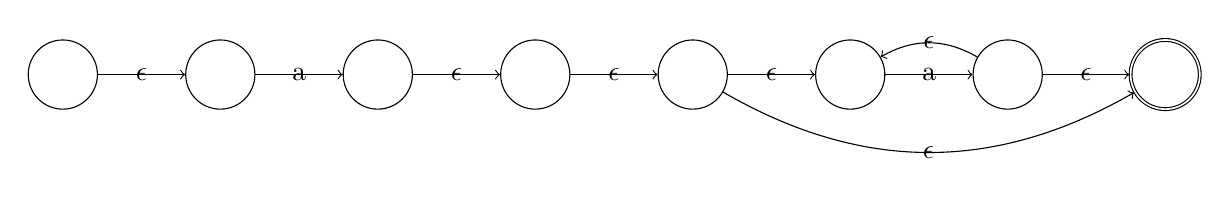
\begin{tikzpicture}
    \node[state](s)                 at (0,0) {};
    \node[state](e0)                at (2,0) {};
    \node[state](a)                 at (4,0) {};
    \node[state](e1)                at (6,0) {};
    \node[state](a*0)               at (8,0) {};
    \node[state](a*1)               at (10,0) {};
    \node[state](a*2)               at (12,0) {};
    \node[accepting, state](a*3)    at (14,0) {};
    % Transitions
    \path
        (s)
            edge [->] node {$\eps$} (e0)
        (e0)
            edge [->] node {a} (a)
        (a) 
            edge [->] node {$\eps$} (e1)
        (e1) 
            edge [->] node {$\eps$} (a*0)
        (a*0)
            edge [->] node {$\eps$} (a*1)
            edge [->, bend right] node {$\eps$} (a*3)
        (a*1) 
            edge [->] node {a} (a*2)
        (a*2)
            edge [->, bend right] node {$\eps$} (a*1)
            edge [->] node {$\eps$} (a*3)
        ;
\end{tikzpicture}\\
\gap
\task{$\beta$}
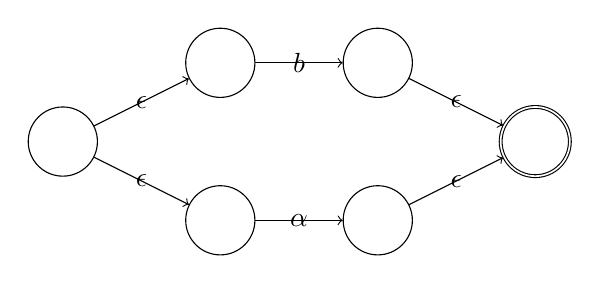
\begin{tikzpicture}
    \node[state](s)                 at (0,0) {};
    \node[state](a0)                at (2,-1) {};
    \node[state](a1)                at (4,-1) {};
    \node[state](b0)                at (2,1) {};
    \node[state](b1)                at (4,1) {};
    \node[accepting, state](e)      at (6,0) {};
    % Transitions
    \path
        (s)
            edge [->] node {$\eps$} (a0)
            edge [->] node {$\eps$} (b0)
        (a0)
            edge [->] node {$\alpha$} (a1)
        (b0)
            edge [->] node {$b$} (b1)
        (a1)
            edge [->] node {$\eps$} (e)
        (b1)
            edge [->] node {$\eps$} (e)
        ;
\end{tikzpicture}\\
\gap
\task{$\gamma$}
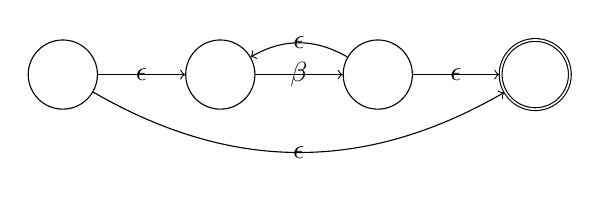
\begin{tikzpicture}
    \node[state](g*0)               at (0,0) {};
    \node[state](g*1)               at (2,0) {};
    \node[state](g*2)               at (4,0) {};
    \node[accepting, state](g*3)    at (6,0) {};
    % Transitions
    \path
        (g*0)
            edge [->] node {$\eps$} (g*1)
            edge [->, bend right] node {$\eps$} (g*3)
        (g*1) 
            edge [->] node {$\beta$} (g*2)
        (g*2)
            edge [->, bend right] node {$\eps$} (g*1)
            edge [->] node {$\eps$} (g*3)
        ;
\end{tikzpicture}\\
\subsection\
\
\end{document}
